% Options for packages loaded elsewhere
\PassOptionsToPackage{unicode}{hyperref}
\PassOptionsToPackage{hyphens}{url}
%
\documentclass[
]{article}
\usepackage{lmodern}
\usepackage{amssymb,amsmath}
\usepackage{ifxetex,ifluatex}
\ifnum 0\ifxetex 1\fi\ifluatex 1\fi=0 % if pdftex
  \usepackage[T1]{fontenc}
  \usepackage[utf8]{inputenc}
  \usepackage{textcomp} % provide euro and other symbols
\else % if luatex or xetex
  \usepackage{unicode-math}
  \defaultfontfeatures{Scale=MatchLowercase}
  \defaultfontfeatures[\rmfamily]{Ligatures=TeX,Scale=1}
\fi
% Use upquote if available, for straight quotes in verbatim environments
\IfFileExists{upquote.sty}{\usepackage{upquote}}{}
\IfFileExists{microtype.sty}{% use microtype if available
  \usepackage[]{microtype}
  \UseMicrotypeSet[protrusion]{basicmath} % disable protrusion for tt fonts
}{}
\makeatletter
\@ifundefined{KOMAClassName}{% if non-KOMA class
  \IfFileExists{parskip.sty}{%
    \usepackage{parskip}
  }{% else
    \setlength{\parindent}{0pt}
    \setlength{\parskip}{6pt plus 2pt minus 1pt}}
}{% if KOMA class
  \KOMAoptions{parskip=half}}
\makeatother
\usepackage{xcolor}
\IfFileExists{xurl.sty}{\usepackage{xurl}}{} % add URL line breaks if available
\IfFileExists{bookmark.sty}{\usepackage{bookmark}}{\usepackage{hyperref}}
\hypersetup{
  pdftitle={The statistical analysis of non-linear longitudinal data in biomedical research using generalized additive models},
  pdfauthor={Ariel Mundo; Timothy J. Muldoon; John R. Tipton},
  hidelinks,
  pdfcreator={LaTeX via pandoc}}
\urlstyle{same} % disable monospaced font for URLs
\usepackage[margin=1in]{geometry}
\usepackage{longtable,booktabs}
% Correct order of tables after \paragraph or \subparagraph
\usepackage{etoolbox}
\makeatletter
\patchcmd\longtable{\par}{\if@noskipsec\mbox{}\fi\par}{}{}
\makeatother
% Allow footnotes in longtable head/foot
\IfFileExists{footnotehyper.sty}{\usepackage{footnotehyper}}{\usepackage{footnote}}
\makesavenoteenv{longtable}
\usepackage{graphicx,grffile}
\makeatletter
\def\maxwidth{\ifdim\Gin@nat@width>\linewidth\linewidth\else\Gin@nat@width\fi}
\def\maxheight{\ifdim\Gin@nat@height>\textheight\textheight\else\Gin@nat@height\fi}
\makeatother
% Scale images if necessary, so that they will not overflow the page
% margins by default, and it is still possible to overwrite the defaults
% using explicit options in \includegraphics[width, height, ...]{}
\setkeys{Gin}{width=\maxwidth,height=\maxheight,keepaspectratio}
% Set default figure placement to htbp
\makeatletter
\def\fps@figure{htbp}
\makeatother
\setlength{\emergencystretch}{3em} % prevent overfull lines
\providecommand{\tightlist}{%
  \setlength{\itemsep}{0pt}\setlength{\parskip}{0pt}}
\setcounter{secnumdepth}{5}
\usepackage{subfig}
\usepackage{breqn}

\title{\textbf{The statistical analysis of non-linear longitudinal data in biomedical research using generalized additive models}}
\usepackage{etoolbox}
\makeatletter
\providecommand{\subtitle}[1]{% add subtitle to \maketitle
  \apptocmd{\@title}{\par {\large #1 \par}}{}{}
}
\makeatother
\subtitle{\emph{Beyond repeated measures ANOVA and Linear Mixed Models}}
\author{Ariel Mundo\footnote{Department of Biomedical Engineering, University of Arkansas, Fayetteville} \and Timothy J. Muldoon\footnote{Department of Biomedical Engineering, University of Arkansas, Fayetteville} \and John R. Tipton\footnote{Department of Mathematical Sciences, University of Arkansas, Fayetteville}}
\date{}

\begin{document}
\maketitle

{
\setcounter{tocdepth}{2}
\tableofcontents
}
\hypertarget{background}{%
\section{Background}\label{background}}

A longitudinal study is designed to repeatedly measure a variable of interest in a group (or groups) of subjects, with the intention of observing the evolution of the treatment effect across time rather than analyzing a single time point (e.g., a cross-sectional study). Medical research commonly uses longitudinal studies to analyze the evolution of patients before, during and after treatment. For example, Sio et. al.~analyzed the evolution of dermatitis symptoms in breast cancer patients after radiotherapy (RT), by taking weekly measurements over the course of two months {[}1{]}, and Kamstra et al measured mouth opening at regular monthly intervals after RT in neck cancer patients {[}2{]}. Other studies using longitudinal designs in biomedical research have tumor analyzed tumor response {[}3--6{]}, antibody expression {[}7,8{]}, and cell metabolism {[}9,10{]}.

Traditionally, a ``frequentist'' or ``classical'' statistical paradigm is used in biomedical research to derive inferences from a longitudinal study. The frequentist paradigm regards probability as a limiting frequency{[}11{]} by assuming a null hypothesis under a statistical model that is often assumed to be an \emph{analysis of variance over repeated measures} (repeated measures ANOVA or rm-ANOVA). The rm-ANOVA model typically makes two key assumptions regarding longitudinal data: constant correlation across same-subject measurements, and observations from each subject are obtained at all time points through the study (a condition also known as \emph{complete observations}) {[}12,13{]}.

The assumption of constant correlation (often known as the \emph{compoun symmetry assumption}) is typically unreasonable because correlation between the measured responses often diminishes as the time interval between the observation increases {[}14{]}.
Due to a variety of causes, the number of observations during a study can vary between all subjects. For example, in a clinical trial voluntary withdrawal from one or multiple patients can occur, whereas attrition in preclinical animal studies due to injury or weight loss is possible. It is even plausible that unexpected complications with equipment or supplies arise that prevent the researcher from collecting measurements at certain time points. In each of these missing data scenarios,the \emph{complete observations} assumption of classical rm-ANOVA is violated.

When incomplete observations occur, a rm-ANOVA model is fit by excluding all subjects with missing observations from the analysis{[}12{]}. This elimination of partially missing data from the analysis can result in increased costs if the desired statistical power is not met with the remaining observations, because it would be necessary to enroll more subjects. At the same time, if the excluded observations contain insightful information that is not used, their elimination from the analysis may limit the demonstration of significant differences between groups. Additionally, rm-ANOVA uses a \emph{post hoc} analysis to assess differences between the measured response in different groups. A \emph{post hoc} analysis is based on multiple repeated comparisons to estimate a \emph{p-value}, a metric that is widely used as a measure of significance. Because the \emph{p-value} is highly variable, multiple comparisons can inflate the false positivity rate (Type I error) {[}15,16{]}, consequently biasing the conclusions of the study. Although corrections exist to address the Type I error issue of multiple comparisons (such as Bonferroni {[}17{]}), they in turn reduce statistical power (\(\alpha\)){[}18{]}, and lead to increased Type II error (fail to reject the null hypothesis although it is false {[}19,20{]}. Therefore, the \emph{post hoc} comparisons commonly used in rm-ANOVA impose a tradeoff between Type I and II errors.

During the last decade, the biomedical community has started to recognize the limitations of rm-ANOVA in the analysis of longitudinal information. The recognition on the limitations of rm-ANOVA is exemplified by the use of linear mixed effects models (LMEMs) by certain groups to analyze longitudinal tumor data {[}10,21{]}. Briefly, LMEMs incorporate \emph{fixed effects}, which correspond to the levels of experimental factors in the study (e.g., the different drug regimens in a clinical trial), and \emph{random effects}, which account for random variation within the population (e.g., the individual-level differences not due to treatment such as weight or age). When compared to the traditional rm-ANOVA, LMEMs are more flexible as they can accommodate missing observations for multiple subjects and allow different modeling strategies for the variability within each measure in every subject {[}22{]}. On the other hand, LMEMs impose restrictions in the distribution of the errors of the random effects, which need to be normally distributed and independent {[}12,23{]}.

One final assumption that is not initially evident for both rm-ANOVA and LMEMs models is that the mean response is expected to change linearly through time{[}22{]}. The linearity assumption in both rm-ANOVA and LMEMs implies that the model is misspecified when the data does not follow a linear trend, which results in unreliable inference. In biomedical research, a particular case of this non-linear behavior in longitudinal data arises in measurements of tumor response in preclinical and clinical settings {[}3,10,21{]}. These studies have shown that the collected signal does not follow a linear trend over time, and presents extreme variability at different time points, making the fit LMEMs or rm-ANOVA model inconsistent with the observed variation. Therefore, when LMEMs and rm-ANOVA are used to draw inference of such highly-variable data the estimates are inevitably biased, because non-linear data is provided to a model which can only accomodate linear trends.

Additionally, although it is possible that a \emph{post hoc} analysis is able to find ``significant'' \emph{p-values}( \emph{p}\textless0.05) the validity of such metric relies on how adequate the model fits the data. In other words, the \emph{p-value} requires that the model and the data have good agreement and if that is not the case, a ``Type 3'' error (known as ``model misspecification'') occurs{[}24{]}. For example, a model that is only able to explain linear responses but is fitted to data that has a quadratic behavior results in \emph{p-values} and parameter estimates that are invalid{[}25{]}.

As the rm-ANOVA and the more flexible LMEM approaches make overly restrictive assumptions regarding the linearity of the response, there is a need for biomedical researchers to explore the use of additional statistical tools that allow the information (and not an assumed behavior) to determine the trend in the data, which enables inference that is appropriate.

In this regard, generalized additive models (GAMs) present an alternative approach to analyze longitudinal data. Although not commonly used in the biomedical community, these non-parametric models have been used to analyze temporal variations in geochemical and palaeoecological data {[}26--28{]}, health-environment interactions {[}29{]} and the dynamics of government in political science {[}30{]} . There are several advantages of GAMs over LMEMs and rm-ANOVA models: GAMs can fit a more flexible class of smooth responses that enable the data to dictate the trend of the model, can easily accommodate missing observations, and can model non-constant correlation between repeated measurements {[}31{]}. Therefore, GAMs can provide a more flexible statistical approach to analyze non-linear biomedical longitudinal data.

The current advances in programming languages designed for statistical analysis (specifically \(\textsf{R}\)), have eased the computational implementation of more complex models beyond LMEMs. In particular, \(\textsf{R}\){[}{\textbf{???}}{]}has an extensive collection of documentation and functions to fit GAMs in the package \emph{mgcv} {[}31,32{]} that not only speed up the initial stages of the analysis but also enable the use of advanced modeling structures (e.g.~hierarchical models, confidence interval comparisons) without requiring advanced programming skills from the user. At the same time, \(\textsf{R}\) has many tools that simplify data simulation, an emerging strategy used to test statistical models {[}33{]}. Data simulation methods allow the researcher to create and explore different alternatives for analysis without collecting information in the field, reducing the time window between experiment design and its implementation, and can be also used for power calculations and study design questions.

This work provides biomedical researchers with a clear understanding of the theory and the practical implementation of GAMs to analyze longitudinal data using by focusing on four areas. First, the limitations of LMEMs and rm-ANOVA regarding missing observations, assumption of linearity of response and constant correlation structures is explained in detail. Second, the key theoretical elements of GAMs are presented using clear and simple mathematical notation while explaining the context and interpretation of the equations. Third, simulated data that reproduces patterns in previously reported studies {[}21{]} is used to illustrate the type of non-linear longitudinal data that often occurs in biomedical research. The simulated data experiments highlight the differences in inference between rm-ANOVA, LMEMs and GAMs on data similar to what is commonly observed in biomedical studies. Finally, reproducibility is emphasized by providing the code to generate the simulated data and the implementation of different models in \(\textsf{R}\), in conjunction with a step-by-step guide demonstrating how to fit models of increasing complexity.

In summary, the exploration of modern statistical techniques to analyze longitudinal data may allow biomedical researchers to consider the use of GAMs instead of rm-ANOVA or LMEMs when the data does not follow a linear trend, and will also help to improve the standards for reproducibility in biomedical research.

\hypertarget{challenges-presented-by-longitudinal-studies}{%
\section{Challenges presented by longitudinal studies}\label{challenges-presented-by-longitudinal-studies}}

\hypertarget{the-repeated-measures-anova}{%
\subsection{The repeated measures ANOVA}\label{the-repeated-measures-anova}}

The \emph{repeated measures analysis of variance} (rm-ANOVA) is the standard statistical analysis for longitudinal data in biomedical research, but certain assumptions are necessary for the model to be valid. From a practical view, the assumptions can be divided in three areas: a linear relationship between covariates and response, a constant correlation between measurements, and complete observations for all subjects. Each one of these assumptions is discussed below.

\hypertarget{linear-relationship}{%
\subsection{Linear relationship}\label{linear-relationship}}

In a biomedical longitudinal study, two or more groups of subjects (patients, mice, samples) are subject to different treatments (e.g., a ``treatment'' group receives a novel drug vs.~a ``control'' group that receives a placebo), and measurements from each subject within each group are collected at specific time points. The collected respnse is modeled with both \emph{fixed} and \emph{random} components. The \emph{fixed} component can be understood as a constant value in the response which the researcher is interested in measuring, i.e, the average effect of the novel drug in the ``treatment'' group. The \emph{random} component can be defined as ``noise'' caused by some inherent variability within the study. For example, if the blood concentration of the drug is measured in certain subjects in the early hours of the morning while others are measured in the afternoon, it is possible that the difference in the collection time of the measurement introduces some ``noise'' in the signal. As their name suggests, this ``random'' variability needs to be modeled as a variable rather than as a constant value.

Mathematically speaking, a rm-ANOVA model with an interaction can be written as:

\begin{equation}
y_{ijt} = \beta_0+ \beta_1 \times time_{t} + \beta_2 \times treatment_{j} + \beta_3 \times time_{t}\times treatment_{j}+\mu_{ij} +\varepsilon_{tij}\\ 
\label{eq:linear-model}
\end{equation}

In this model \(y_{ijt}\) is the response by subject \(i\), in treatment group \(j\) at time \(t\), which can be decomposed in a mean value \(\beta_0\), \emph{fixed effects} of time (\(time_t\)), treatment (\(treatment_j\)) and their interaction \(time_t*treatment_j\) which have linear slopes given by \(\beta_1, \beta_2\) and \(\beta_3\), respectively. The \emph{random effect} \(\mu_{ij}\), accounts for variability in each subject within each group by allowing different values for each subject. Independent errors \(\varepsilon_{tij}\) represent random variation not explained by the \emph{fixed} or \emph{random} effects.
In a biomedical research context, suppose two treatments groups are used in a study (e.g., ``placebo'' vs.~``novel drug'' or ``saline'' vs.~``chemotherapy''). Then, the group terms in Equation \eqref{eq:linear-model} can be written as below with \(j=0\) representing the first treatment group (Group A) and \(j=1\) representing the second treatment group (Group B). The linear models then can be expressed as

\begin{equation}
y_{ijt} = \begin{cases}
\beta_0 + \beta_1\times time_{t}+\mu_{ijt}+\varepsilon_{ijt}   & \mbox{if Group A}\\
\beta_0 + \beta_1 \times time_{t} + \beta_2 \times treatment_{j} +\beta_3 \times time_{t} \times treatment_{j}+\mu_{ijt}+\varepsilon_{ijt}  & \mbox{if Group B}\\
\end{cases}
\label{eq:ANOVA-by-group}
\end{equation}

To further simplify the expression, substitute \(\widetilde{\mu}=\beta_0+\beta_{2}\) and \(\widetilde{\beta_{1}}=\beta_{1}+\beta_{3}\) in the equation for Group B. This substitution allows for a different intercept and slope for Group B. The model is written as

\begin{equation}
y_{ijt} = \begin{cases}
\beta_0 + \beta_1\times time_{t}+\mu_{ijt}+\varepsilon_{ijt}   & \mbox{if Group A}\\
\widetilde{\mu} + \widetilde{\beta_1} \times time_{t} +\mu_{ijt}+\varepsilon_{ijt}  & \mbox{if Group B}\\
\end{cases}
\label{eq:ANOVA-lines}
\end{equation}

Presenting the model in this manner makes clear that when treating different groups, an rm-ANOVA model is able to accommodate non-parallel lines in each case (different intercepts and slopes per group). In other words, When it is stated that an rm-ANOVA model ``expects'' a linear relationship between the covariates and the response, this means that either presented as Equation \eqref{eq:linear-model}, Equation \eqref{eq:ANOVA-by-group} or Equation \eqref{eq:ANOVA-lines}, an rm-ANOVA model is only able to accommodate linear patterns in the data. If the data show non-linear behavior, the rm-ANOVa model will approximate this behavior with non-parallel lines. Because the construction of the model is essentially the same in LMEMs, the linearity assumption holds for these models, although it is possible to fit models with different slopes at the subject-level{[}22{]}.

When the data does not follow a linear trend, the fit that an rm-ANOVA or LMEM produces may not accurately represent the trends in the data. To demonstrate this inaccurate representation, longitudinal data where a normally distributed response of two groups of 10 subjects each is simulated, and a rm-ANOVA model (Equation \eqref{eq:linear-model}) is fitted to the data using \(\textsf{R}\){[}{\textbf{???}}{]} and the package \emph{nlme}{[}{\textbf{???}}{]} (code in the Appendix). Briefly, two cases for the mean responses for each group are considered: in the first case, the mean response in each group is a linear function with different intercepts and slopes (negative slope for Group 1 and positive slope for Group 2 ). In the second case, a quadratic function is used for the mean response per group (concave down for Group 1 and concave up for Group 2 ). From the mean response per group in the linear or quadratic case, individual responses for each subject in each group are simulated using covariance matrices for with compound symmetry (constant variance across time) or independent errors (errors that are generated from a a normal distribution but are not constant over time). Thus, the response per subject corresponds to the mean response per group plus the error (compound symmetry or independent). To this data, an rm-ANOVA model identical as Equation @ref:eqn(linear-model) is fitted. The resulting simulated data, simulated errors, individual response and fitted parameters from the model are plotted.

\begin{figure}
\centering
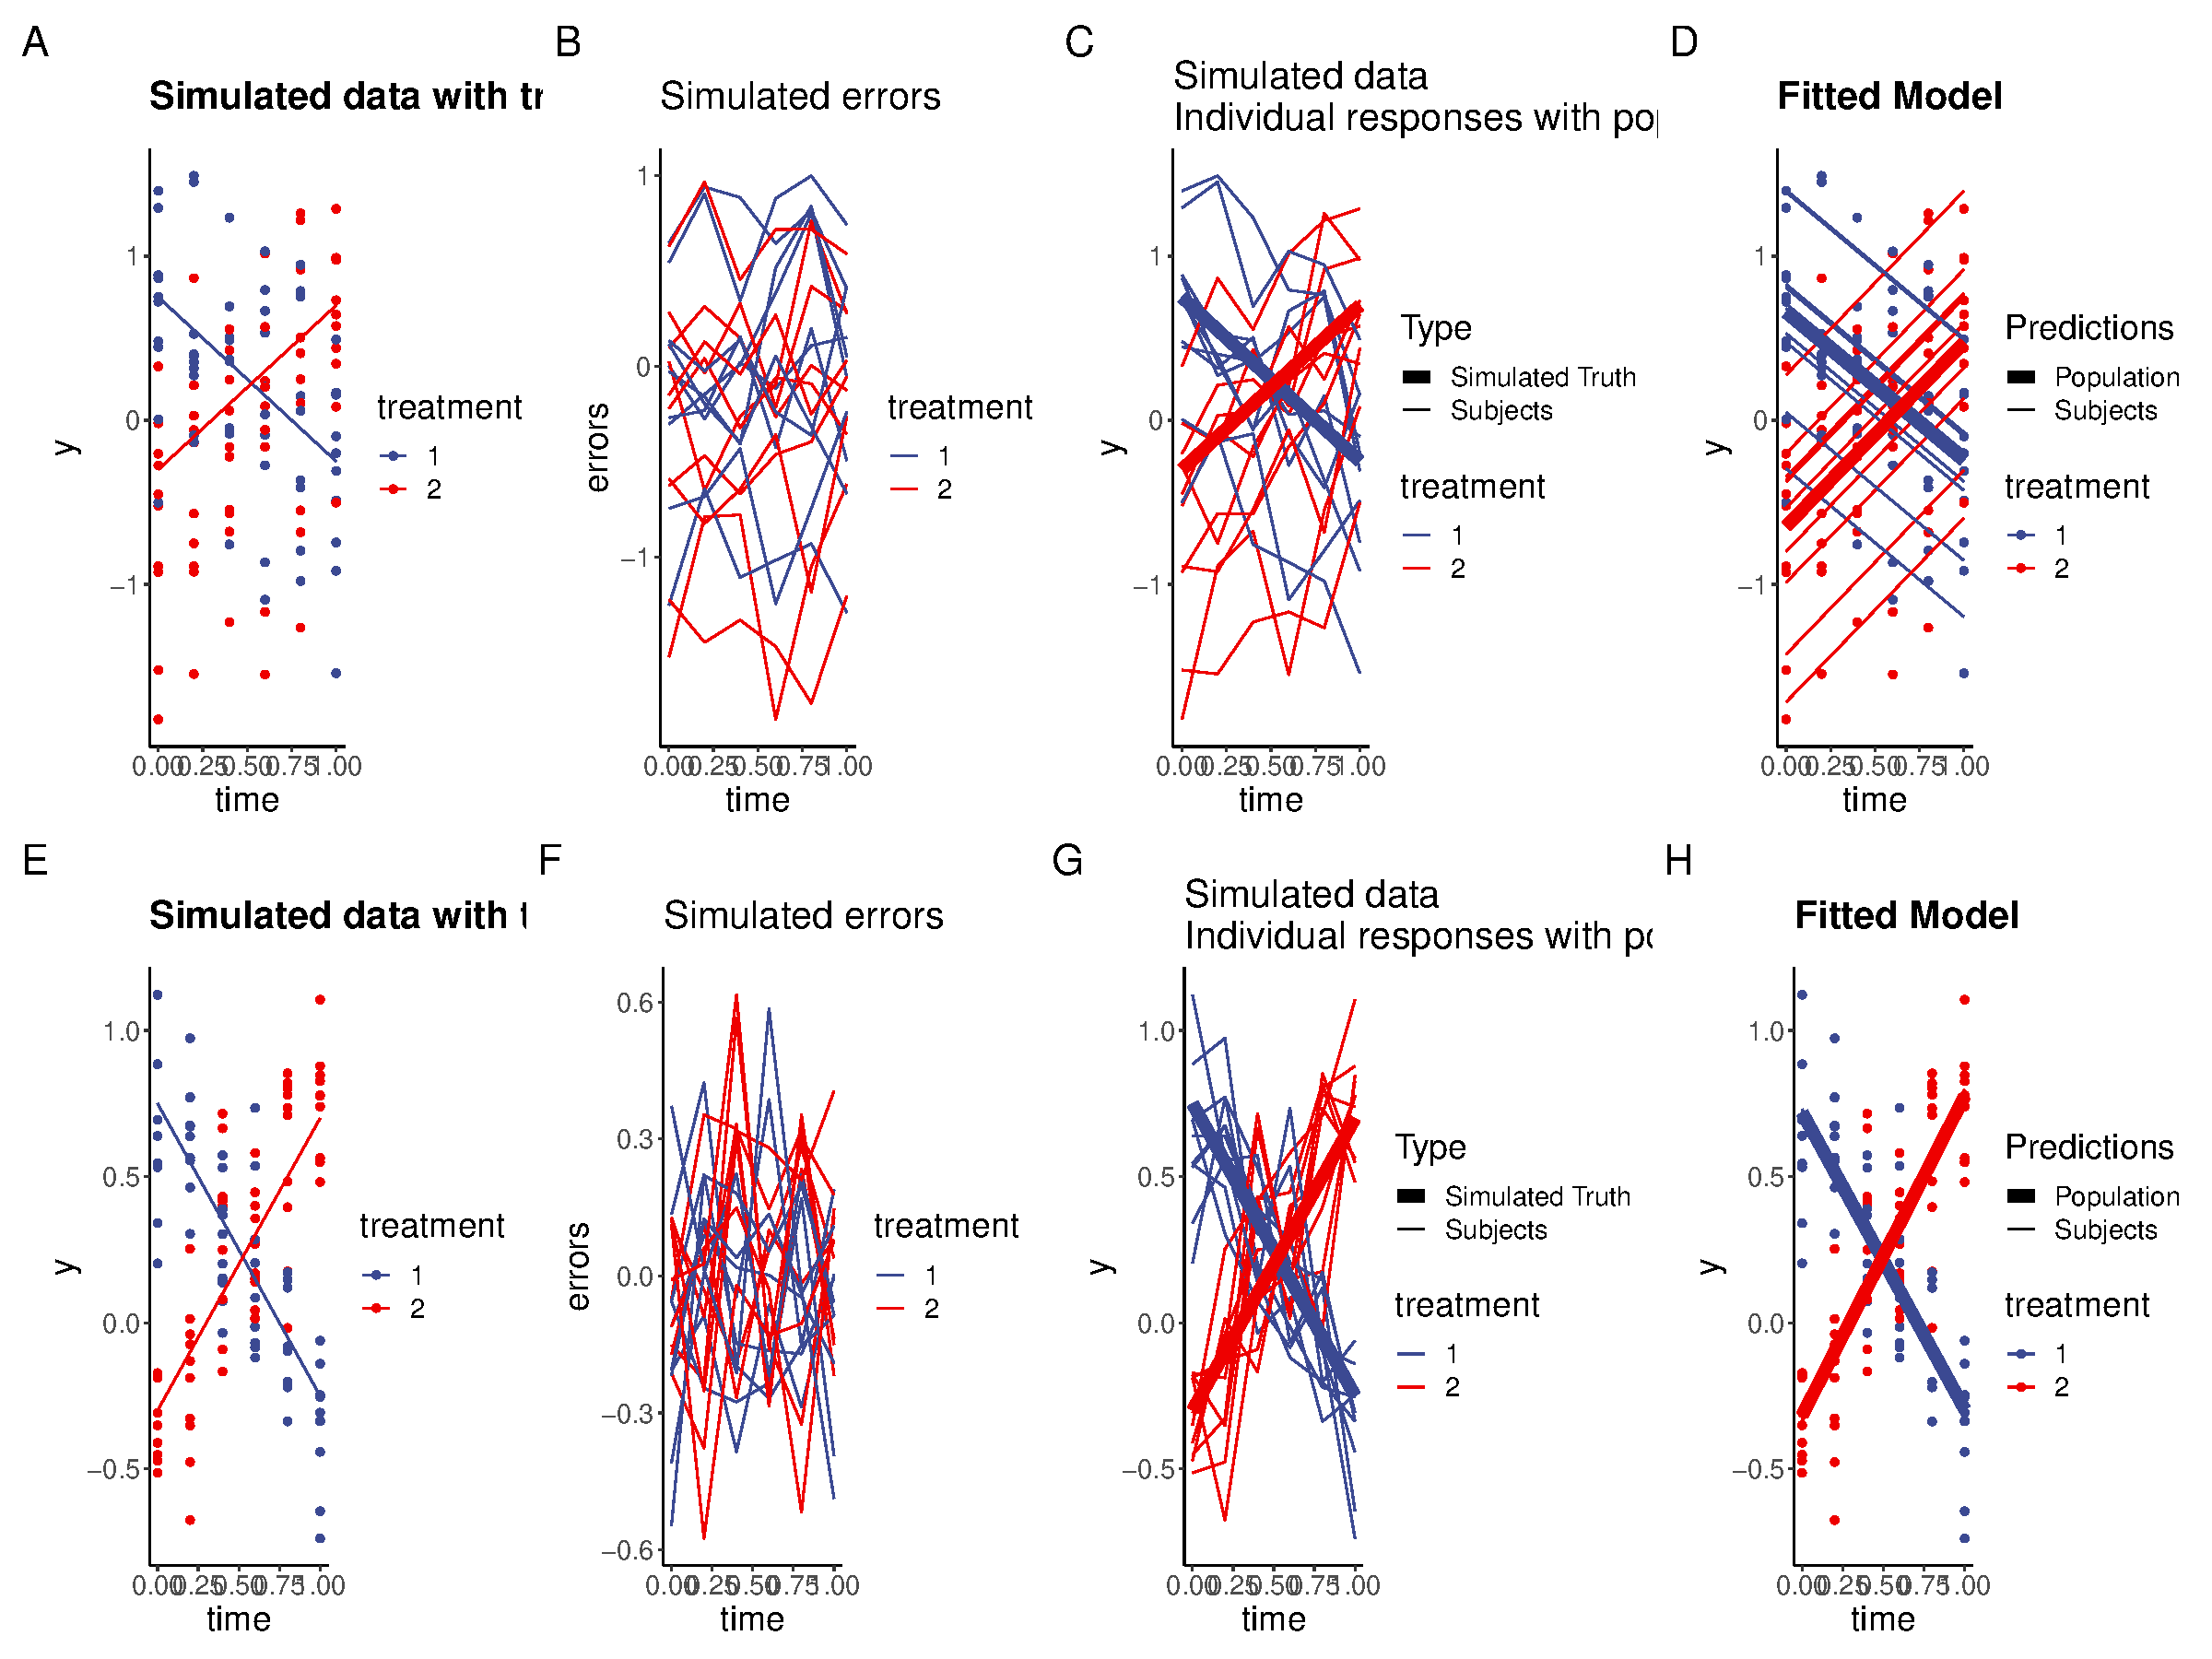
\includegraphics{Manuscript_AM_v2_files/figure-latex/linear-models-1.pdf}
\caption{\label{fig:linear-models}Simulated linear responses from two groups with a rm-ANOVA model fitted. Top row, simulated data, lines represent mean response. Bottom row, fitted model, thick lines represent predicted mean response}
\end{figure}

It is clear from Figure \ref{fig:linear-models} that the fit produced by the rm-ANOVA model is good as the predictions for the mean response are reasonably close to the ``truth'' of the simulated data.

However, consider the case when the data follows a non-linear trend, such as the simulated data in Figure \ref{fig:quadratic-response}. Here, the simulated data follows a quadratic behavior. The figure shows that changes in each group occur through the timeline, although the final mean value is the same as the initial value. Fitting an rm-ANOVA model \eqref{eq:linear-model} to this data produces the fit that appears at the bottom right of Figure \ref{fig:quadratic-response}.

\begin{figure}
\centering
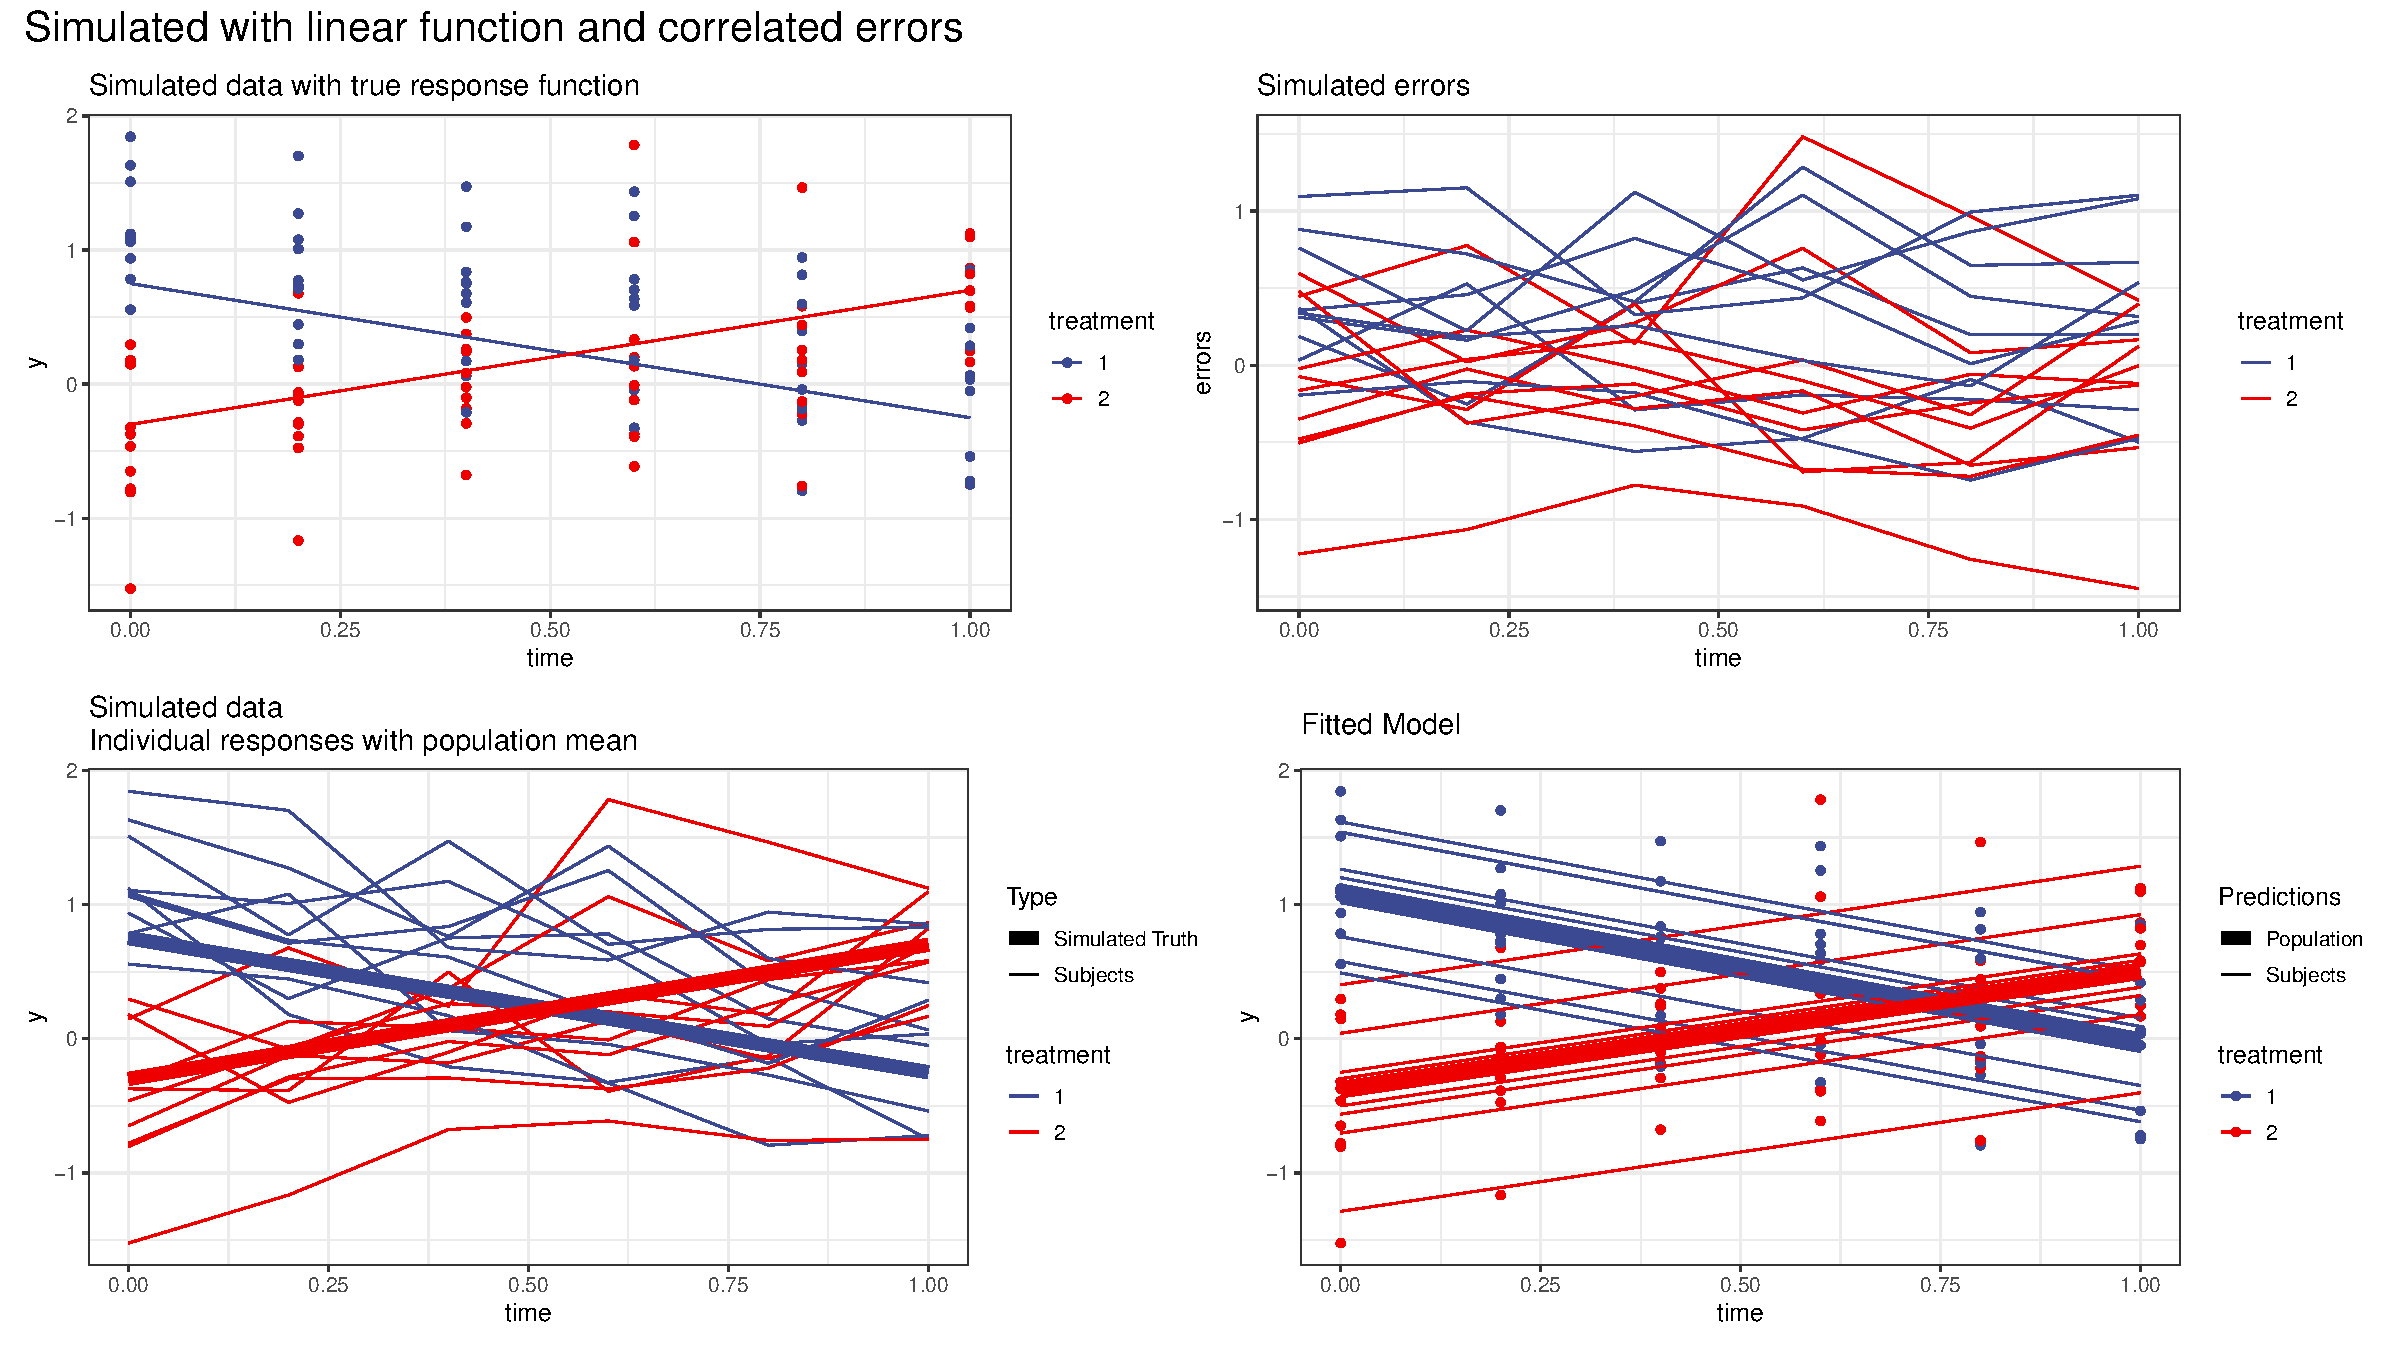
\includegraphics{Manuscript_AM_v2_files/figure-latex/quadratic-response-1.pdf}
\caption{\label{fig:quadratic-response}Simulated quadratic responses from two groups with a rm-ANOVA model fitted. Top row, simulated data, lines represent mean response. Bottom row, fitted model, thick lines represent predicted mean response}
\end{figure}

In this case, compare the predictions to the simulated data and it is noticeable that the model is not capturing the changes within each group throughout the timeline. This highlights the limitation of rm-ANOVA and LMEMs with longitudinal non-linear data, where the model is only flexible enough to allow different slopes per group, but is unable to follow any trend that is highly variable.

\hypertarget{covariance-in-rm-anova-and-lmems}{%
\subsection{Covariance in rm-ANOVA and LMEMs}\label{covariance-in-rm-anova-and-lmems}}

In a longitudinal study there is an expected \emph{variance} between repeated measurements on the same subject, and because repeated measures occur in the subjects within each group, there is a \emph{covariance} between measurements at each time point within each group. The \emph{covariance matrix} (also known as the variance-covariance matrix) is a matrix that captures the variation between and within subjects in a longitudinal study{[}34{]} (For an in-depth analysis of the covariance matrix see {[}35,36{]}).

In the case of an rm-ANOVA analysis, it is typically assumed that the covariance matrix has a specific construction known as \emph{compound symmetry} (also known as ``sphericity'' or ``circularity''). Under this assumption, the between-subject variance and within-subject correlation are constant across time {[}36--38{]}. However, it has been shown that this condition is frequently unjustified because the correlation between measurements tends to change over time {[}39{]}; and it is higher between consecutive measurements {[}12,14{]}. A visual representation of the
Although corrections can be made (such as Huyhn-Feldt or Greenhouse-Geisser) the effectiveness of each correction is limited because it depends on the size of the sample,the number of repeated measurements{[}33{]}, and they are not robust if the group sizes are unbalanced {[}40{]}. In other words, if the data does not present constant correlation between repeated measurements, the assumptions required for an rm-ANOVA model are not met and the use of corrections may still not provide a reasonable adjustment that makes the model valid.

In the case of LMEMs, one key advantage over rm-ANOVA is that they allow different structures for the variance-covariance matrix including exponential, autoregressive of order 1, rational quadratic and others {[}22{]}. Nevertheless, the analysis required to determine an appropriate variance-covariance structure for the data can be a long process by itself. Overall, the spherical assumption for rm-ANOVA may not capture the natural variations of the correlation in the data, and can bias the inferences from the analysis.

\hypertarget{missing-observations}{%
\subsection{Missing observations}\label{missing-observations}}

Missing observations are an issue that arises frequently in longitudinal studies. In biomedical research, this situation can be caused by reasons beyond the control of the investigator {[}41{]}. Dropout from patients, attrition or injury in animals are among the reasons for missing observations. Statistically, missing information can be classified as \emph{missing at random} (MAR), \emph{missing completely at random} (MCAR), and \emph{missing not at random} (MNAR) {[}36{]}. In a MAR scenario, the pattern of the missing information is related to some variable in the data, but it is not related to the variable of interest {[}42{]}. If the data are MCAR, this means that the missigness is completely unrelated to the collected information {[}43{]}, and in the case of MNAR the missing values are dependent on their value. An rm-ANOVA model assumes complete observations for all subjects, and therefore subjects with one or more missing observations are excluded from the analysis. This is inconvenient because the remaining subjects might not accurately represent the population, and statistical power is affected by this reduction in sample size {[}44{]}.

In the case of LMEMs, inferences from the model are valid when missing observations in the data exist that are MAR or MCAR {[}35{]}. The pattern of missing observations can be considered MAR if the missing observations are not related any of the other variables measured in the study {[}39{]}. For example, if attrition occurs in all mice that had lower weights at the beginning of a chemotherapy response study, the missing data can be considered MAR because the missigness is unrelated to other variables of interest.

This section has presented the assumptions of rm-ANOVA to analyze longitudinal information and its differences when compared to LMEMs regarding to missing data and the modeling of the covariance matrix. Of notice, LMEMs offer a more robust and flexible approach than rm-ANOVA and if the data follows a linear trend, they provide an excellent choice to derive inferences from a repeated measures study. However, when the data presents high variability, LMEMs fail to capture the non-linear trend of the data. To analyze such type of data, we present generalized additive models (GAMs) as an alternative in the following section.

\hypertarget{gams-as-a-special-case-of-generalized-linear-models}{%
\section{GAMs as a special case of Generalized Linear Models}\label{gams-as-a-special-case-of-generalized-linear-models}}

\hypertarget{gams-and-basis-functions}{%
\subsection{GAMs and Basis Functions}\label{gams-and-basis-functions}}

A GAM is a special case of the Generalized Linear Model (GLM), a framework that allows for response distributions that do not follow a normal distribution {[}31,45{]}. Following the notation by Simpson {[}28{]} A GAM model can be represented as:

\begin{equation}
  y_{ijt}=\beta_0+f(x_t\mid \beta)+\varepsilon_{ijt}
  \label{eq:GAM}
\end{equation}

Where \(y_{ijt}\) is the response at time \(t\), \(\beta_0\) is the expected value at time 0, the change of \(y_{ijt}\) over time is represented by the function \(f(x_t\mid \beta)\) and \(\varepsilon_{ijt}\) represents the residuals.

In contrast to rm-ANOVA or LMEMs, GAMs use \emph{smooth functions} to model the relationship between the covariates and the response. This approach is more advantageous as it does not restrict the model to a linear relationship. One possible function for \(f(x_t\mid \beta)\) that allows for non-linear responses is a polynomial, but a major limitation is that they create a ``global'' fit as they assume that the same relationship exists everywhere, which can cause problems with the fit {[}30{]}.In particular, as \(t\) goes to \(\pm \infty\), \(f(x_t \mid \beta)\) goes to \(\pm \infty\) which is almost always unrealistic.

The model specification for GAMs requires that the \emph{smooth functions} are represented in a parametric way that fit within the GLM framework, and this step is achieved by using \emph{basis functions} to represent them. A \emph{basis} is a set of functions that capture the space where the smooths that approximate \(f(x_t \mid \beta)\) exist {[}28{]}. For the linear model in \eqref{eq:linear-model}, the basis coefficients are \(\beta_1\), \(\beta_2\) and \(\beta_3\) and the basis vectors are \(time_t\), \(treatment_j\) and \(time_t \times treatment_j\). The basis function then, is the combination of basis coefficients and basis vectors that map the possible relationship between the covariates and the response {[}46{]}, which in the case of \eqref{eq:linear-model} is restricted to a linear behavior. In the case of \eqref{eq:GAM}, the basis function is \(f(x_t\mid \beta)\), which means that the model allows relationships beyond linear for the covariates.

In GAMs the \emph{basis functions} are represented over evenly spaced ranges of the covariates known as \emph{knots}. A commonly used \emph{basis function} is a cubic spline, which is a smooth curve constructed from cubic polynomials joined together at the knot locations{[}28,31{]}. Cubic splines have a long history in solving non-parametric statistical problems and are often a default choice to fit GAMs as they are a simple, flexible and powerful option to obtain visual smoothness {[}47{]}. Therefore, GAMs overcome the limitation that occurs in LMEMs and rm-ANOVA when the data is non linear, such as Figure \ref{fig:quadratic-response}. Regarding longitudinal data, Pedersen et al {[}27{]} demonstrated the capabilities of GAMs in this area using ecological data.

The use of GAMs to analyze biomedical longitudinal data, and the impact of missing observations in the fit of the model will be examined in detail in the following section using simulation.

\begin{center}\rule{0.5\linewidth}{0.5pt}\end{center}

\hypertarget{references}{%
\section*{References}\label{references}}
\addcontentsline{toc}{section}{References}

\hypertarget{refs}{}
\leavevmode\hypertarget{ref-sio2016}{}%
{[}1{]} T.T. Sio, P.J. Atherton, B.J. Birckhead, D.J. Schwartz, J.A. Sloan, D.K. Seisler, J.A. Martenson, C.L. Loprinzi, P.C. Griffin, R.F. Morton, others, Repeated measures analyses of dermatitis symptom evolution in breast cancer patients receiving radiotherapy in a phase 3 randomized trial of mometasone furoate vs placebo (N06C4 {[}alliance{]}), Supportive Care in Cancer. 24 (2016) 3847--3855.

\leavevmode\hypertarget{ref-kamstra2015}{}%
{[}2{]} J. Kamstra, P. Dijkstra, M. Van Leeuwen, J. Roodenburg, J. Langendijk, Mouth opening in patients irradiated for head and neck cancer: A prospective repeated measures study, Oral Oncology. 51 (2015) 548--555.

\leavevmode\hypertarget{ref-roblyer2011}{}%
{[}3{]} D. Roblyer, S. Ueda, A. Cerussi, W. Tanamai, A. Durkin, R. Mehta, D. Hsiang, J.A. Butler, C. McLaren, W.-P. Chen, others, Optical imaging of breast cancer oxyhemoglobin flare correlates with neoadjuvant chemotherapy response one day after starting treatment, Proceedings of the National Academy of Sciences. 108 (2011) 14626--14631.

\leavevmode\hypertarget{ref-tank2020}{}%
{[}4{]} A. Tank, H.M. Peterson, V. Pera, S. Tabassum, A. Leproux, T. O'Sullivan, E. Jones, H. Cabral, N. Ko, R.S. Mehta, others, Diffuse optical spectroscopic imaging reveals distinct early breast tumor hemodynamic responses to metronomic and maximum tolerated dose regimens, Breast Cancer Research. 22 (2020) 1--10.

\leavevmode\hypertarget{ref-pavlov2018}{}%
{[}5{]} M.V. Pavlov, T.I. Kalganova, Y.S. Lyubimtseva, V.I. Plekhanov, G.Y. Golubyatnikov, O.Y. Ilyinskaya, A.G. Orlova, P.V. Subochev, D.V. Safonov, N.M. Shakhova, others, Multimodal approach in assessment of the response of breast cancer to neoadjuvant chemotherapy, Journal of Biomedical Optics. 23 (2018) 091410.

\leavevmode\hypertarget{ref-demidov2018}{}%
{[}6{]} V. Demidov, A. Maeda, M. Sugita, V. Madge, S. Sadanand, C. Flueraru, I.A. Vitkin, Preclinical longitudinal imaging of tumor microvascular radiobiological response with functional optical coherence tomography, Scientific Reports. 8 (2018) 1--12.

\leavevmode\hypertarget{ref-ritter2001}{}%
{[}7{]} G. Ritter, L.S. Cohen, C. Williams, E.C. Richards, L.J. Old, S. Welt, Serological analysis of human anti-human antibody responses in colon cancer patients treated with repeated doses of humanized monoclonal antibody a33, Cancer Research. 61 (2001) 6851--6859.

\leavevmode\hypertarget{ref-roth2017}{}%
{[}8{]} E.M. Roth, A.C. Goldberg, A.L. Catapano, A. Torri, G.D. Yancopoulos, N. Stahl, A. Brunet, G. Lecorps, H.M. Colhoun, Antidrug antibodies in patients treated with alirocumab, (2017).

\leavevmode\hypertarget{ref-jones2018}{}%
{[}9{]} J.D. Jones, H.E. Ramser, A.E. Woessner, K.P. Quinn, In vivo multiphoton microscopy detects longitudinal metabolic changes associated with delayed skin wound healing, Communications Biology. 1 (2018) 1--8.

\leavevmode\hypertarget{ref-skala2010}{}%
{[}10{]} M.C. Skala, A.N. Fontanella, L. Lan, J.A. Izatt, M.W. Dewhirst, Longitudinal optical imaging of tumor metabolism and hemodynamics, Journal of Biomedical Optics. 15 (2010) 011112.

\leavevmode\hypertarget{ref-wagenmakers2008}{}%
{[}11{]} E.-J. Wagenmakers, M. Lee, T. Lodewyckx, G.J. Iverson, Bayesian versus frequentist inference, in: Bayesian Evaluation of Informative Hypotheses, Springer, 2008: pp. 181--207.

\leavevmode\hypertarget{ref-gueorguieva2004}{}%
{[}12{]} R. Gueorguieva, J.H. Krystal, Move over anova: Progress in analyzing repeated-measures data andits reflection in papers published in the archives of general psychiatry, Archives of General Psychiatry. 61 (2004) 310--317.

\leavevmode\hypertarget{ref-schober2018}{}%
{[}13{]} P. Schober, T.R. Vetter, Repeated measures designs and analysis of longitudinal data: If at first you do not succeed---try, try again, Anesthesia and Analgesia. 127 (2018) 569.

\leavevmode\hypertarget{ref-ugrinowitsch2004}{}%
{[}14{]} C. Ugrinowitsch, G.W. Fellingham, M.D. Ricard, Limitations of ordinary least squares models in analyzing repeated measures data, Medicine and Science in Sports and Exercise. 36 (2004) 2144--2148.

\leavevmode\hypertarget{ref-liu2010}{}%
{[}15{]} C. Liu, T.P. Cripe, M.-O. Kim, Statistical issues in longitudinal data analysis for treatment efficacy studies in the biomedical sciences, Molecular Therapy. 18 (2010) 1724--1730.

\leavevmode\hypertarget{ref-halsey2015}{}%
{[}16{]} L.G. Halsey, D. Curran-Everett, S.L. Vowler, G.B. Drummond, The fickle p value generates irreproducible results, Nature Methods. 12 (2015) 179--185.

\leavevmode\hypertarget{ref-abdi2010}{}%
{[}17{]} H. Abdi, Holm's sequential bonferroni procedure, Encyclopedia of Research Design. 1 (2010) 1--8.

\leavevmode\hypertarget{ref-nakagawa2004}{}%
{[}18{]} S. Nakagawa, A farewell to bonferroni: The problems of low statistical power and publication bias, Behavioral Ecology. 15 (2004) 1044--1045.

\leavevmode\hypertarget{ref-gelman2012}{}%
{[}19{]} A. Gelman, J. Hill, M. Yajima, Why we (usually) don't have to worry about multiple comparisons, Journal of Research on Educational Effectiveness. 5 (2012) 189--211.

\leavevmode\hypertarget{ref-albers2019}{}%
{[}20{]} C. Albers, The problem with unadjusted multiple and sequential statistical testing, Nature Communications. 10 (2019) 1--4.

\leavevmode\hypertarget{ref-vishwanath2009}{}%
{[}21{]} K. Vishwanath, H. Yuan, W.T. Barry, M.W. Dewhirst, N. Ramanujam, Using optical spectroscopy to longitudinally monitor physiological changes within solid tumors, Neoplasia. 11 (2009) 889--900.

\leavevmode\hypertarget{ref-pinheiro2006}{}%
{[}22{]} J. Pinheiro, D. Bates, Mixed-effects models in s and s-plus, Springer Science \& Business Media, 2006.

\leavevmode\hypertarget{ref-barr2013}{}%
{[}23{]} D.J. Barr, R. Levy, C. Scheepers, H.J. Tily, Random effects structure for confirmatory hypothesis testing: Keep it maximal, Journal of Memory and Language. 68 (2013) 255--278.

\leavevmode\hypertarget{ref-dennis2019}{}%
{[}24{]} B. Dennis, J.M. Ponciano, M.L. Taper, S.R. Lele, Errors in statistical inference under model misspecification: Evidence, hypothesis testing, and aic, Frontiers in Ecology and Evolution. 7 (2019) 372.

\leavevmode\hypertarget{ref-wang2019}{}%
{[}25{]} B. Wang, Z. Zhou, H. Wang, X.M. Tu, C. Feng, The p-value and model specification in statistics, General Psychiatry. 32 (2019).

\leavevmode\hypertarget{ref-rose2012}{}%
{[}26{]} N.L. Rose, H. Yang, S.D. Turner, G.L. Simpson, An assessment of the mechanisms for the transfer of lead and mercury from atmospherically contaminated organic soils to lake sediments with particular reference to Scotland, UK, Geochimica et Cosmochimica Acta. 82 (2012) 113--135.

\leavevmode\hypertarget{ref-pedersen2019}{}%
{[}27{]} E.J. Pedersen, D.L. Miller, G.L. Simpson, N. Ross, Hierarchical generalized additive models in ecology: An introduction with mgcv, PeerJ. 7 (2019) e6876.

\leavevmode\hypertarget{ref-simpson2018}{}%
{[}28{]} G.L. Simpson, Modelling palaeoecological time series using generalised additive models, Frontiers in Ecology and Evolution. 6 (2018) 149.

\leavevmode\hypertarget{ref-yang2012}{}%
{[}29{]} L. Yang, G. Qin, N. Zhao, C. Wang, G. Song, Using a generalized additive model with autoregressive terms to study the effects of daily temperature on mortality, BMC Medical Research Methodology. 12 (2012) 165.

\leavevmode\hypertarget{ref-beck1998}{}%
{[}30{]} N. Beck, S. Jackman, Beyond linearity by default: Generalized additive models, American Journal of Political Science. (1998) 596--627.

\leavevmode\hypertarget{ref-wood2017}{}%
{[}31{]} S.N. Wood, Generalized additive models: An introduction with r, CRC press, 2017.

\leavevmode\hypertarget{ref-wood2016}{}%
{[}32{]} S.N. Wood, N., Pya, B. Säfken, Smoothing parameter and model selection for general smooth models (with discussion), Journal of the American Statistical Association. 111 (2016) 1548--1575.

\leavevmode\hypertarget{ref-haverkamp2017}{}%
{[}33{]} N. Haverkamp, A. Beauducel, Violation of the sphericity assumption and its effect on type-i error rates in repeated measures anova and multi-level linear models (mlm), Frontiers in Psychology. 8 (2017) 1841.

\leavevmode\hypertarget{ref-wolfinger1996}{}%
{[}34{]} R.D. Wolfinger, Heterogeneous variance: Covariance structures for repeated measures, Journal of Agricultural, Biological, and Environmental Statistics. (1996) 205--230.

\leavevmode\hypertarget{ref-west2014}{}%
{[}35{]} B.T. West, K.B. Welch, A.T. Galecki, Linear mixed models: A practical guide using statistical software, CRC Press, 2014.

\leavevmode\hypertarget{ref-weiss2005}{}%
{[}36{]} R.E. Weiss, Modeling longitudinal data, Springer Science \& Business Media, 2005.

\leavevmode\hypertarget{ref-geisser1958}{}%
{[}37{]} S. Geisser, S.W. Greenhouse, others, An extension of box's results on the use of the \(F\) distribution in multivariate analysis, The Annals of Mathematical Statistics. 29 (1958) 885--891.

\leavevmode\hypertarget{ref-huynh1976}{}%
{[}38{]} H. Huynh, L.S. Feldt, Estimation of the box correction for degrees of freedom from sample data in randomized block and split-plot designs, Journal of Educational Statistics. 1 (1976) 69--82.

\leavevmode\hypertarget{ref-maxwell2017}{}%
{[}39{]} S.E. Maxwell, H.D. Delaney, K. Kelley, Designing experiments and analyzing data: A model comparison perspective, Routledge, 2017.

\leavevmode\hypertarget{ref-keselman2001}{}%
{[}40{]} H. Keselman, J. Algina, R.K. Kowalchuk, The analysis of repeated measures designs: A review, British Journal of Mathematical and Statistical Psychology. 54 (2001) 1--20.

\leavevmode\hypertarget{ref-molenberghs2004}{}%
{[}41{]} G. Molenberghs, H. Thijs, I. Jansen, C. Beunckens, M.G. Kenward, C. Mallinckrodt, R.J. Carroll, Analyzing incomplete longitudinal clinical trial data, Biostatistics. 5 (2004) 445--464.

\leavevmode\hypertarget{ref-scheffer2002}{}%
{[}42{]} J. Scheffer, Dealing with missing data, (2002).

\leavevmode\hypertarget{ref-potthoff2006}{}%
{[}43{]} R.F. Potthoff, G.E. Tudor, K.S. Pieper, V. Hasselblad, Can one assess whether missing data are missing at random in medical studies?, Statistical Methods in Medical Research. 15 (2006) 213--234.

\leavevmode\hypertarget{ref-ma2012}{}%
{[}44{]} Y. Ma, M. Mazumdar, S.G. Memtsoudis, Beyond repeated-measures analysis of variance: Advanced statistical methods for the analysis of longitudinal data in anesthesia research, Regional Anesthesia \& Pain Medicine. 37 (2012) 99--105.

\leavevmode\hypertarget{ref-hastie1987}{}%
{[}45{]} T. Hastie, R. Tibshirani, Generalized additive models: Some applications, Journal of the American Statistical Association. 82 (1987) 371--386.

\leavevmode\hypertarget{ref-hefley2017}{}%
{[}46{]} T.J. Hefley, K.M. Broms, B.M. Brost, F.E. Buderman, S.L. Kay, H.R. Scharf, J.R. Tipton, P.J. Williams, M.B. Hooten, The basis function approach for modeling autocorrelation in ecological data, Ecology. 98 (2017) 632--646.

\leavevmode\hypertarget{ref-wegman1983}{}%
{[}47{]} E.J. Wegman, I.W. Wright, Splines in statistics, Journal of the American Statistical Association. 78 (1983) 351--365.

\end{document}
